
% Prepared by Calvin Kent
%
% Assignment Template v19.02
%
%%% 20xx0x/MATHxxx/Crowdmark/Ax
%
\documentclass[12pt]{article} %
\usepackage{amsthm}
\usepackage{CKpreamble}
\usepackage{CKassignment}
\usepackage{mdframed}
\usepackage{euscript}
\usepackage{tikz}
\usepackage{pgfplots}

%
\begin{document}
	\pagenumbering{arabic}
	% Start of class settings ...
	\renewcommand*{\coursecode}{MATH 235} % renew course code
	\renewcommand*{\assgnnumber}{Assignment 1} % renew assignment number
	\renewcommand*{\submdate}{September 14, 2021} % renew the date
	\renewcommand*{\studentfname}{Abdullah} % Student first name
	\renewcommand*{\studentlname}{Zubair} % Student last name
    \renewcommand*{\proofname}{Proof:}
	% \renewcommand*{\studentnum}{20836288} % Student number

	\renewcommand\qedsymbol{$\blacksquare$}
	\setfigpath
	% End of class settings	
	% \pagestyle{crowdmark}
	\newgeometry{left=18mm, right=18mm, top=22mm, bottom=22mm} % page is set to default values
	\fancyhfoffset[L,O]{0pt} % header orientation fixed
	% End of class settings
	%%% Note to user:
	% CTRL + F <CHANGE ME:> (without the angular brackets) in CKpreamble to specify graphics paths accordingly.
	% The command \circled[]{} accepts one optional and one mandatory argument.
	% Optional argument is for the size of the circle and mandatory argument is for its contents.
	% \circled{A} produces circled A, with size drawn for letter A. \circled[TT]{A} produces circled A with size drawn for TT.
	% https://github.com/CalvinKent/My-LaTeX
	%%%

	%%%%%%%%%%%%%%%%%%%%%%%%%%%%%%%%%%%%%%%%%%%%%%%%%%%%%%%%%%%%%%%%%%%%%%%%%%%%%%%
	%%%                        CUSTOM MACRO VIM-TEX                             %%%
	%%       call IMAP('NOM', '\nomenclature{}', 'tex')               

	%%%%%%%%%%%%%%%%%%%%%%%%%%%%%%%%%%%%%%%%%%%%%%%%%%%%%%%%%%%%%%%%%%%%%%%%%%%%%%%

	% Crowdmark assignment start
	% qnumber, qname, points

\begin{center}
	\textbf{\underline{\Huge{Lecture 3 - Homework}}}
\end{center}
\begin{qstn}
  Let $f \colon \R \to \R$, $f(x) = x$. Is $f$ the identity function on $\R$? Justify your answer.
\end{qstn}
\begin{qstn}
  For each of the following, you are given a function and its mapping diagram. For each question,
  \begin{itemize}
    \item State weather the function is invertible, if not then weather it is injective or surjective or neither,
      with justification.
    \item Determine the range of the function.
  \end{itemize}
  \begin{enumerate}[label=(\alph*)]
    \item $g \colon \mathcal{A} \to \mathcal{B}$,
    \begin{center}
     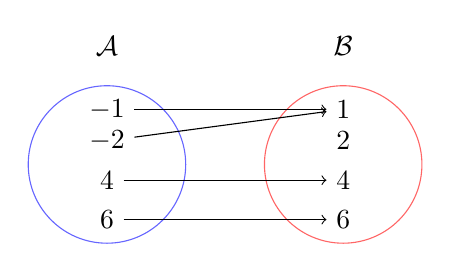
\begin{tikzpicture}
        % draw the sets
        \filldraw[fill=white!20, draw=blue!60] (-1.5,0) circle (1cm);
        \filldraw[fill=white!20, draw=red!60] (1.5,0) circle (1cm);


        % the texts
        \node at (-1.5,1.5) {$\mathcal{A}$};
        \node at (1.5,1.5) {$\mathcal{B}$};

        % the points in the sets (here I just create nodes to use them later on to position
        % the circles and the arrows
        \node (x1) at (-1.5,0.7) {$-1$};
        \node (x2) at (-1.5,0.3) {$-2$};
        \node (x3) at (-1.5,-0.2) {$4$};
        \node (x4) at (-1.5,-0.7) {$6$};
        \node (y1) at (1.5,0.7) {$1$};
        \node (y2) at (1.5,0.3) {$2$};
        \node (y3) at (1.5,-0.2) {$4$};
        \node (y4) at (1.5,-0.7) {$6$};

        % draw the arrows
        \draw[->] (x1) -- (y1);
        \draw[->] (x2) -- (y1);
        \draw[->] (x3) -- (y3);
        \draw[->] (x4) -- (y4);

    \end{tikzpicture}
  \end{center}


  \item $f \colon \EuScript{H} \to \EuScript{T}$,
    \begin{center}
     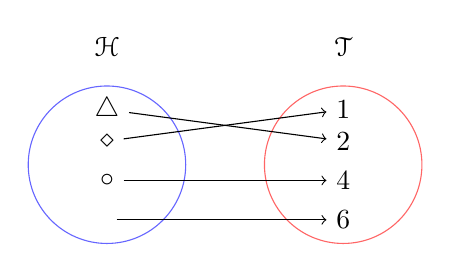
\begin{tikzpicture}
        % draw the sets
        \filldraw[fill=white!20, draw=blue!60] (-1.5,0) circle (1cm);
        \filldraw[fill=white!20, draw=red!60] (1.5,0) circle (1cm);


        % the texts
        \node at (-1.5,1.5) {$\EuScript{H}$};
        \node at (1.5,1.5) {$\EuScript{T}$};

        % the points in the sets (here I just create nodes to use them later on to position
        % the circles and the arrows
        \node (x1) at (-1.5,0.7) {$\triangle$};
        \node (x2) at (-1.5,0.3) {$\diamond$};
        \node (x3) at (-1.5,-0.2) {$\circ$};
        \node (x4) at (-1.5,-0.7) {$\square$};
        \node (y1) at (1.5,0.7) {$1$};
        \node (y2) at (1.5,0.3) {$2$};
        \node (y3) at (1.5,-0.2) {$4$};
        \node (y4) at (1.5,-0.7) {$6$};

        % draw the arrows
        \draw[->] (x2) -- (y1);
        \draw[->] (x1) -- (y2);
        \draw[->] (x3) -- (y3);
        \draw[->] (x4) -- (y4);

    \end{tikzpicture}
  \end{center}

  \item $T \colon \mathcal{V} \to \mathcal{W}$,
    \begin{center}
     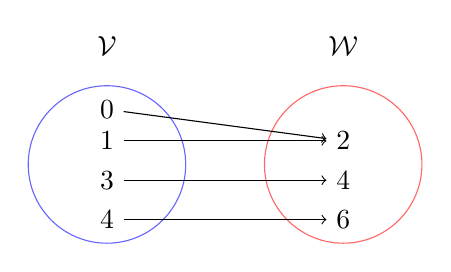
\begin{tikzpicture}
        % draw the sets
        \filldraw[fill=white!20, draw=blue!60] (-1.5,0) circle (1cm);
        \filldraw[fill=white!20, draw=red!60] (1.5,0) circle (1cm);


        % the texts
        \node at (-1.5,1.5) {$\mathcal{V}$};
        \node at (1.5,1.5) {$\mathcal{W}$};

        % the points in the sets (here I just create nodes to use them later on to position
        % the circles and the arrows
        \node (x1) at (-1.5,0.7) {$0$};
        \node (x2) at (-1.5,0.3) {$1$};
        \node (x3) at (-1.5,-0.2) {$3$};
        \node (x4) at (-1.5,-0.7) {$4$};
        \node (y2) at (1.5,0.3) {$2$};
        \node (y3) at (1.5,-0.2) {$4$};
        \node (y4) at (1.5,-0.7) {$6$};

        % draw the arrows
        \draw[->] (x1) -- (y2);
        \draw[->] (x2) -- (y2);
        \draw[->] (x3) -- (y3);
        \draw[->] (x4) -- (y4);

    \end{tikzpicture}
  \end{center}


  \item $S \colon \mathcal{Q} \to \mathcal{P}$,
    \begin{center}
     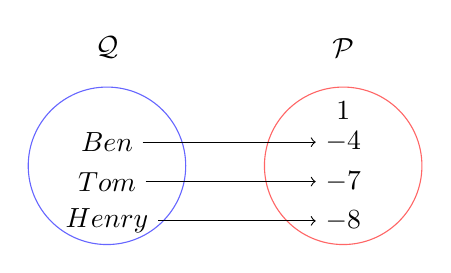
\begin{tikzpicture}
        % draw the sets
        \filldraw[fill=white!20, draw=blue!60] (-1.5,0) circle (1cm);
        \filldraw[fill=white!20, draw=red!60] (1.5,0) circle (1cm);


        % the texts
        \node at (-1.5,1.5) {$\mathcal{Q}$};
        \node at (1.5,1.5) {$\mathcal{P}$};

        % the points in the sets (here I just create nodes to use them later on to position
        % the circles and the arrows
        \node (x1) at (-1.5,0.3) {$\text{Ben}$};
        \node (x3) at (-1.5,-0.2) {$\text{Tom}$};
        \node (x4) at (-1.5,-0.7) {$\text{Henry}$};
        \node (y1) at (1.5,0.7) {$1$};
        \node (y2) at (1.5,0.3) {$-4$};
        \node (y3) at (1.5,-0.2) {$-7$};
        \node (y4) at (1.5,-0.7) {$-8$};

        % draw the arrows
        \draw[->] (x1) -- (y2);
        \draw[->] (x3) -- (y3);
        \draw[->] (x4) -- (y4);

    \end{tikzpicture}
  \end{center}

  \newpage

  \item $P \colon \mathcal{D} \to \mathcal{C}$,
    \begin{center}
     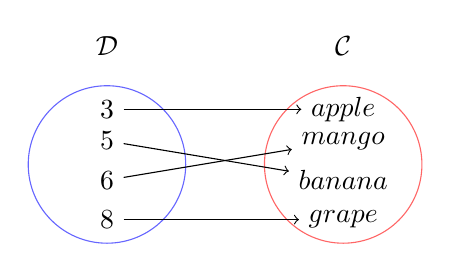
\begin{tikzpicture}
        % draw the sets
        \filldraw[fill=white!20, draw=blue!60] (-1.5,0) circle (1cm);
        \filldraw[fill=white!20, draw=red!60] (1.5,0) circle (1cm);


        % the texts
        \node at (-1.5,1.5) {$\mathcal{D}$};
        \node at (1.5,1.5) {$\mathcal{C}$};

        % the points in the sets (here I just create nodes to use them later on to position
        % the circles and the arrows
        \node (x1) at (-1.5,0.7) {$3$};
        \node (x2) at (-1.5,0.3) {$5$};
        \node (x3) at (-1.5,-0.2) {$6$};
        \node (x4) at (-1.5,-0.7) {$8$};
        \node (y1) at (1.5,0.7) {$\text{apple}$};
        \node (y2) at (1.5,0.3) {$\text{mango}$};
        \node (y3) at (1.5,-0.2) {$\text{banana}$};
        \node (y4) at (1.5,-0.7) {$\text{grape}$};

        % draw the arrows
        \draw[->] (x1) -- (y1);
        \draw[->] (x2) -- (y3);
        \draw[->] (x3) -- (y2);
        \draw[->] (x4) -- (y4);

    \end{tikzpicture}
  \end{center}


  \end{enumerate}
\end{qstn}


\begin{qstn}
  Is the function defined in Example 3.2 an invertible function? Justify your answer.
\end{qstn}

\begin{qstn}
  Let $\mathcal{A} = \{-1,3,4,6,7\}$ and $\mathcal{B} = \{6,-1,4,3,7\} $ be sets. Come up with an invertible function between the
  two sets and prove that your function is invertible.
\end{qstn}

\begin{qstn}
  Let $\mathcal{A}$ and $\mathcal{B}$ be sets. Let $T \colon \mathcal{A} \to \mathcal{B}$ be an invertible function.
  Let $\mathcal{R}_T$ be the range of $T$, is it true that $\mathcal{B} = \mathcal{R}_T$? Justify your answer.
  \textbf{(This is a very important question)}
\end{qstn}

\begin{qstn}
  Let $ \mathcal{X} = \{1,4,9,36\} $ and $ \mathcal{Y} = \{1,2,3,6\} $ be sets, lets define the
  following function, 
  \begin{itemize}
    \item $\mathcal{L} \colon \mathcal{A} \to \mathcal{B}$.
    \item $\mathcal{L}(x) = \sqrt{x} $.
  \end{itemize}
  Prove that $\mathcal{L}$ is invertible.
\end{qstn}

\begin{qstn}
  Let $ \mathcal{X} = \{-1,0,1,2,3\} $ and $ \mathcal{Y} = \{10,2,5,1\} $ be sets, lets define the
  following function, 
  \begin{itemize}
    \item $\mathcal{P} \colon \mathcal{A} \to \mathcal{B}$.
    \item $\mathcal{P}(x) = x^2 +  1 $.
  \end{itemize}
  Prove that $\mathcal{P}$ is \textbf{not }invertible.
\end{qstn}



\end{document}




























